% Options for packages loaded elsewhere
\PassOptionsToPackage{unicode}{hyperref}
\PassOptionsToPackage{hyphens}{url}
%
\documentclass[
]{article}
\usepackage{amsmath,amssymb}
\usepackage{iftex}
\ifPDFTeX
  \usepackage[T1]{fontenc}
  \usepackage[utf8]{inputenc}
  \usepackage{textcomp} % provide euro and other symbols
\else % if luatex or xetex
  \usepackage{unicode-math} % this also loads fontspec
  \defaultfontfeatures{Scale=MatchLowercase}
  \defaultfontfeatures[\rmfamily]{Ligatures=TeX,Scale=1}
\fi
\usepackage{lmodern}
\ifPDFTeX\else
  % xetex/luatex font selection
\fi
% Use upquote if available, for straight quotes in verbatim environments
\IfFileExists{upquote.sty}{\usepackage{upquote}}{}
\IfFileExists{microtype.sty}{% use microtype if available
  \usepackage[]{microtype}
  \UseMicrotypeSet[protrusion]{basicmath} % disable protrusion for tt fonts
}{}
\makeatletter
\@ifundefined{KOMAClassName}{% if non-KOMA class
  \IfFileExists{parskip.sty}{%
    \usepackage{parskip}
  }{% else
    \setlength{\parindent}{0pt}
    \setlength{\parskip}{6pt plus 2pt minus 1pt}}
}{% if KOMA class
  \KOMAoptions{parskip=half}}
\makeatother
\usepackage{xcolor}
\usepackage[margin=1in]{geometry}
\usepackage{graphicx}
\makeatletter
\def\maxwidth{\ifdim\Gin@nat@width>\linewidth\linewidth\else\Gin@nat@width\fi}
\def\maxheight{\ifdim\Gin@nat@height>\textheight\textheight\else\Gin@nat@height\fi}
\makeatother
% Scale images if necessary, so that they will not overflow the page
% margins by default, and it is still possible to overwrite the defaults
% using explicit options in \includegraphics[width, height, ...]{}
\setkeys{Gin}{width=\maxwidth,height=\maxheight,keepaspectratio}
% Set default figure placement to htbp
\makeatletter
\def\fps@figure{htbp}
\makeatother
\setlength{\emergencystretch}{3em} % prevent overfull lines
\providecommand{\tightlist}{%
  \setlength{\itemsep}{0pt}\setlength{\parskip}{0pt}}
\setcounter{secnumdepth}{5}
\usepackage{caption}
\usepackage{subcaption}
\usepackage{multirow}
\usepackage{float}
\restylefloat{table}
\let\oldtable\table
\let\endoldtable\endtable
\renewenvironment{table}[1][H]{\oldtable[H]}{\endoldtable}
\usepackage{fancyhdr}
\pagestyle{fancy}
\fancyhf{}
\fancyhead[L]{\textbf{2025-05-24}}
\fancyhead[C]{\textbf{Econometrics Problem Set 2}}
\fancyhead[R]{\textbf{Gereon Staratschek}}
\fancyfoot[C]{\thepage}
\usepackage{booktabs}
\usepackage{longtable}
\usepackage{array}
\usepackage{multirow}
\usepackage{wrapfig}
\usepackage{float}
\usepackage{colortbl}
\usepackage{pdflscape}
\usepackage{tabu}
\usepackage{threeparttable}
\usepackage{threeparttablex}
\usepackage[normalem]{ulem}
\usepackage{makecell}
\usepackage{xcolor}
\ifLuaTeX
  \usepackage{selnolig}  % disable illegal ligatures
\fi
\usepackage{bookmark}
\IfFileExists{xurl.sty}{\usepackage{xurl}}{} % add URL line breaks if available
\urlstyle{same}
\hypersetup{
  pdftitle={Macroeconometrics - UK variables report},
  pdfauthor={Souleymane Faye \& Gereon Staratschek},
  hidelinks,
  pdfcreator={LaTeX via pandoc}}

\title{Macroeconometrics - UK variables report}
\author{Souleymane Faye \& Gereon Staratschek}
\date{2025-05-24}

\begin{document}
\maketitle

\section*{Preliminaries}

In this project, we aim to analyze the development of the Gross Domestic
Product (GDP), exchange rates, and trade balance of the United Kingdom
(UK). We collect our data from the OECD open data portal. We use data on
a quarterly basis, starting latest in 1997. This period covers important
financial events such as the Global Financial Crisis (GFC) in 2007, the
Brexit referendum in 2016 and UK's final EU leave in 2020 as well as the
COVID-19 pandemic from 2020-2022.

\section*{Exercise 1 -  Univariate Analysis}

\subsection*{Part 1: Analyzing the time series in levels}

Looking at the plain time series data and analyzing the plots, we get
the following results:

\begin{figure}

{\centering \includegraphics[width=0.8\linewidth]{../figures/uk_levels_base_plot} 

}

\caption{Residual diagnostics from ARIMA(1,0,4).}\label{fig:resid-plot}
\end{figure}

\textbf{GDP}: Data on UK's GDP is available on a quarterly basis
starting in 1955. GDP exhibits a clear, upwards trend with only a few
shocks (such as the 2020 COVID-19 oandemic or the 2007 financial crisis)
interrupting the general trend. Hence, the GDP of the UK is clearly not
stationary. However, the trend seems to be linear, suggesting that the
first-differences time series of the GDP might be stationary.
\textbackslash{}

\textbf{Trade Balance}: As GDP, data on the trade balance is available
on a quarterly basis starting in 1955. We see that the trade balance
fluctuates around 0 until the 1990s where a negative trend seems to set
in continueing until the 2010s, when trade balance starts fluctuating
around a low, negative value. However, since the observed spikes are
getting much bigger over time, we also see an increase in fluctuation
around the respective stationary mean. Hence, the data seems to be
stationary in the beginning and in the end with a negative trend being
observed between the 1990s and the 2010s. \textbackslash{}

\textbf{Exchange Rate}: Data on the exchange rate is available since
1997 on a quarterly basis. It exhibits stationarity between 1997 and
2007, as well as from 2007 onwards. In 2007, a shock seems to have
shifted the mean of the stationary process downwards.

\subsection*{Part 2: Conducting unit roots and stationarity tests}

In this section, we aim to formally conduct stationarity tests for the
series. As explained in the last section, we have reason to doubt that
our series are entirely stationary. However, for our analysis, we are
relying on stationarity properties of the series. Hence, after
identifying the non-stationary series formally, we will conduct the
first-difference transformation to obtain stationary series for our
analysis.\textbackslash{}

Starting with the non-transformed series, we run a series of tests for
each time series separately
(\textcolor{red}{Explain the type of tests here!}) \textbackslash{}

\textbf{GDP}:

\bgroup \table[H]
\centering
\caption{\label{tab:unnamed-chunk-2}Unit-root and stationarity tests for UK GDP}
\centering
\begin{tabular}[t]{lrrrrr}
\toprule
\multicolumn{1}{c}{ } & \multicolumn{2}{c}{ADF} & \multicolumn{1}{c}{KPSS} \\
\cmidrule(l{3pt}r{3pt}){2-3} \cmidrule(l{3pt}r{3pt}){4-4}
test & statistic & p.value & crit\_10pct & crit\_5pct & crit\_1pct\\
\midrule
ADF & -2.530635 & 0.3525184 & NA & NA & NA\\
KPSS & 4.731673 & 0.0100000 & NA & NA & NA\\
ERS DF-GLS & 3.073724 & NA & -1.62 & -1.94 & -2.57\\
PP & -21.532938 & 0.0483211 & NA & NA & NA\\
\bottomrule
\end{tabular}
\endtable\egroup

\textbf{Trade Balance}:

\bgroup \table[H]
\centering
\caption{\label{tab:unnamed-chunk-3}Unit-root and stationarity tests for UK GDP}
\centering
\begin{tabular}[t]{lrrrrr}
\toprule
\multicolumn{1}{c}{ } & \multicolumn{2}{c}{ADF} & \multicolumn{1}{c}{KPSS} \\
\cmidrule(l{3pt}r{3pt}){2-3} \cmidrule(l{3pt}r{3pt}){4-4}
test & statistic & p.value & crit\_10pct & crit\_5pct & crit\_1pct\\
\midrule
ADF & -2.2250155 & 0.4812789 & NA & NA & NA\\
KPSS & 3.3948515 & 0.0100000 & NA & NA & NA\\
ERS DF-GLS & -0.6723293 & NA & -1.62 & -1.94 & -2.57\\
PP & -157.4146465 & 0.0100000 & NA & NA & NA\\
\bottomrule
\end{tabular}
\endtable\egroup

\textbf{Exchange Rate}:

\bgroup \table[H]
\centering
\caption{\label{tab:unnamed-chunk-4}Unit-root and stationarity tests for UK GDP}
\centering
\begin{tabular}[t]{lrrrrr}
\toprule
\multicolumn{1}{c}{ } & \multicolumn{2}{c}{ADF} & \multicolumn{1}{c}{KPSS} \\
\cmidrule(l{3pt}r{3pt}){2-3} \cmidrule(l{3pt}r{3pt}){4-4}
test & statistic & p.value & crit\_10pct & crit\_5pct & crit\_1pct\\
\midrule
ADF & -2.382354 & 0.4179499 & NA & NA & NA\\
KPSS & 1.754143 & 0.0100000 & NA & NA & NA\\
ERS DF-GLS & -1.414941 & NA & -1.62 & -1.94 & -2.58\\
PP & -13.157562 & 0.3539359 & NA & NA & NA\\
\bottomrule
\end{tabular}
\endtable\egroup

\textbackslash{} \textcolor{red}{Interprete these results!}
\textbackslash{}

Now, let us turn to the first-difference transformations of the time
series. \textbackslash{}

\textbf{GDP}:

\bgroup \table[H]
\centering
\caption{\label{tab:unnamed-chunk-5}Unit-root and stationarity tests for UK GDP}
\centering
\begin{tabular}[t]{lrrrrr}
\toprule
\multicolumn{1}{c}{ } & \multicolumn{2}{c}{ADF} & \multicolumn{1}{c}{KPSS} \\
\cmidrule(l{3pt}r{3pt}){2-3} \cmidrule(l{3pt}r{3pt}){4-4}
test & statistic & p.value & crit\_10pct & crit\_5pct & crit\_1pct\\
\midrule
ADF & -8.0195142 & 0.01 & NA & NA & NA\\
KPSS & 0.0864308 & 0.10 & NA & NA & NA\\
ERS DF-GLS & -7.9411516 & NA & -1.62 & -1.94 & -2.57\\
PP & -321.6127812 & 0.01 & NA & NA & NA\\
\bottomrule
\end{tabular}
\endtable\egroup

\textbf{Trade Balance}:

\bgroup \table[H]
\centering
\caption{\label{tab:unnamed-chunk-6}Unit-root and stationarity tests for UK Trade Balance}
\centering
\begin{tabular}[t]{lrrrrr}
\toprule
\multicolumn{1}{c}{ } & \multicolumn{2}{c}{ADF} & \multicolumn{1}{c}{KPSS} \\
\cmidrule(l{3pt}r{3pt}){2-3} \cmidrule(l{3pt}r{3pt}){4-4}
test & statistic & p.value & crit\_10pct & crit\_5pct & crit\_1pct\\
\midrule
ADF & -8.1714448 & 0.01 & NA & NA & NA\\
KPSS & 0.0349289 & 0.10 & NA & NA & NA\\
ERS DF-GLS & -12.9115650 & NA & -1.62 & -1.94 & -2.57\\
PP & -300.0884288 & 0.01 & NA & NA & NA\\
\bottomrule
\end{tabular}
\endtable\egroup

\textbf{Exchange Rate}:

\bgroup \table[H]
\centering
\caption{\label{tab:unnamed-chunk-7}Unit-root and stationarity tests for UK Exchange Rate}
\centering
\begin{tabular}[t]{lrrrrr}
\toprule
\multicolumn{1}{c}{ } & \multicolumn{2}{c}{ADF} & \multicolumn{1}{c}{KPSS} \\
\cmidrule(l{3pt}r{3pt}){2-3} \cmidrule(l{3pt}r{3pt}){4-4}
test & statistic & p.value & crit\_10pct & crit\_5pct & crit\_1pct\\
\midrule
ADF & -5.0408902 & 0.01 & NA & NA & NA\\
KPSS & 0.0837118 & 0.10 & NA & NA & NA\\
ERS DF-GLS & -2.1882524 & NA & -1.62 & -1.94 & -2.58\\
PP & -82.8852407 & 0.01 & NA & NA & NA\\
\bottomrule
\end{tabular}
\endtable\egroup

\subsection*{Part 3: Model Estimation}

\textbf{GDP}: For the GDP, we use the stationary first-differenced data.
Our tests suggest an ARIMA(1,0,4) process:

\begin{figure}

{\centering 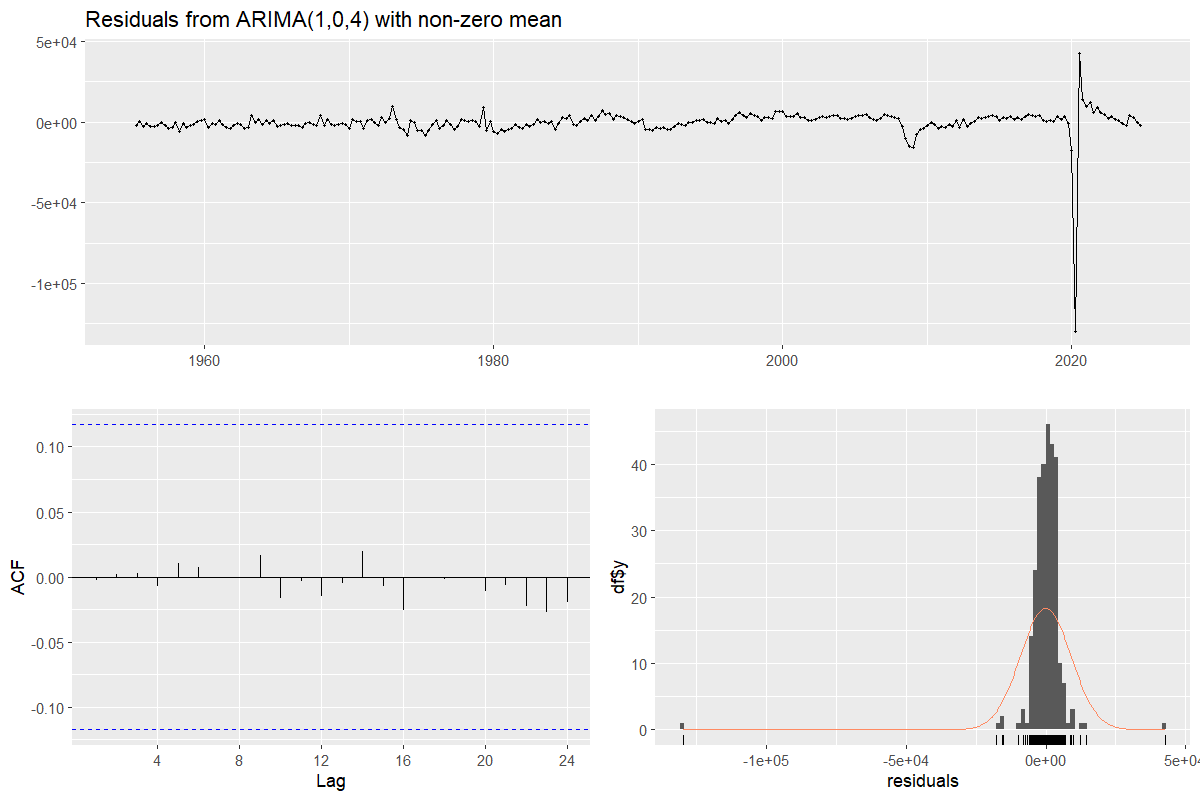
\includegraphics[width=0.8\linewidth]{../results/GDP (first-differenced)_residuals} 

}

\caption{Model estimation - GDP}\label{fig:unnamed-chunk-8}
\end{figure}

The coefficients of the model are as follows:

\bgroup \table[H]
\centering
\caption{\label{tab:unnamed-chunk-9}Model coefficients GDP}
\centering
\begin{tabular}[t]{lrr}
\toprule
term & estimate & std.error\\
\midrule
ar1 & 0.4886750 & 0.2015697\\
ma1 & -0.7703784 & 0.1988893\\
ma2 & 0.0925464 & 0.0930497\\
ma3 & 0.1352912 & 0.0747171\\
ma4 & -0.2405810 & 0.0610664\\
\addlinespace
intercept & 1832.9872955 & 232.7539989\\
\bottomrule
\end{tabular}
\endtable\egroup

\textbf{Trade Balance}: For the Trade Balance, we use the stationary
level data. Our tests suggests an ARIMA(0,0,4) process:

\begin{figure}

{\centering 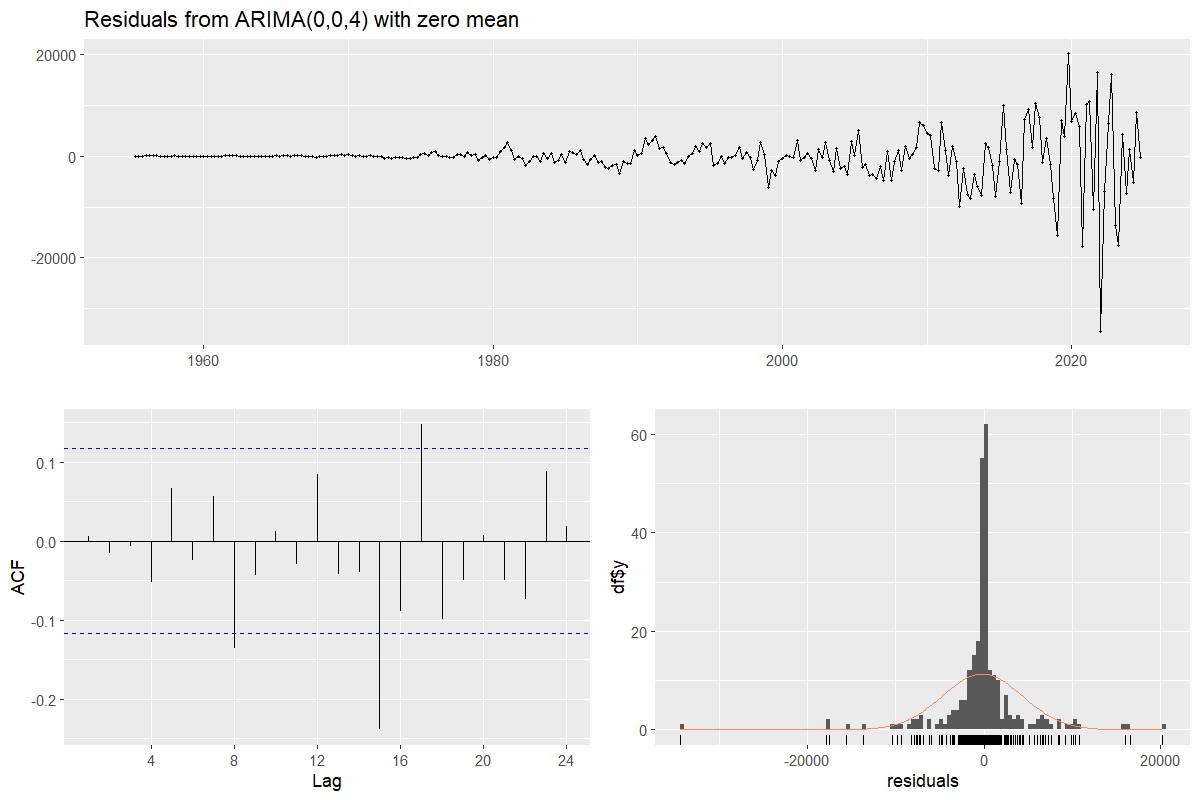
\includegraphics[width=0.8\linewidth]{../results/Trade Balance_residuals} 

}

\caption{Model estimation - Trade Balance}\label{fig:unnamed-chunk-10}
\end{figure}

The coefficients of the model are as follows:

\bgroup \table[H]
\centering
\caption{\label{tab:unnamed-chunk-11}Model coefficients Trade Balance}
\centering
\begin{tabular}[t]{lrr}
\toprule
term & estimate & std.error\\
\midrule
ma1 & -0.7749122 & 0.0571450\\
ma2 & -0.1000937 & 0.0735727\\
ma3 & -0.0300321 & 0.0804010\\
ma4 & 0.2784463 & 0.0640672\\
\bottomrule
\end{tabular}
\endtable\egroup

\textbf{Exchange rate}: For the Exchange Rate, we use te stationary
level data. Our tests suggests an ARIMA(1,0,0) process:

\begin{figure}

{\centering 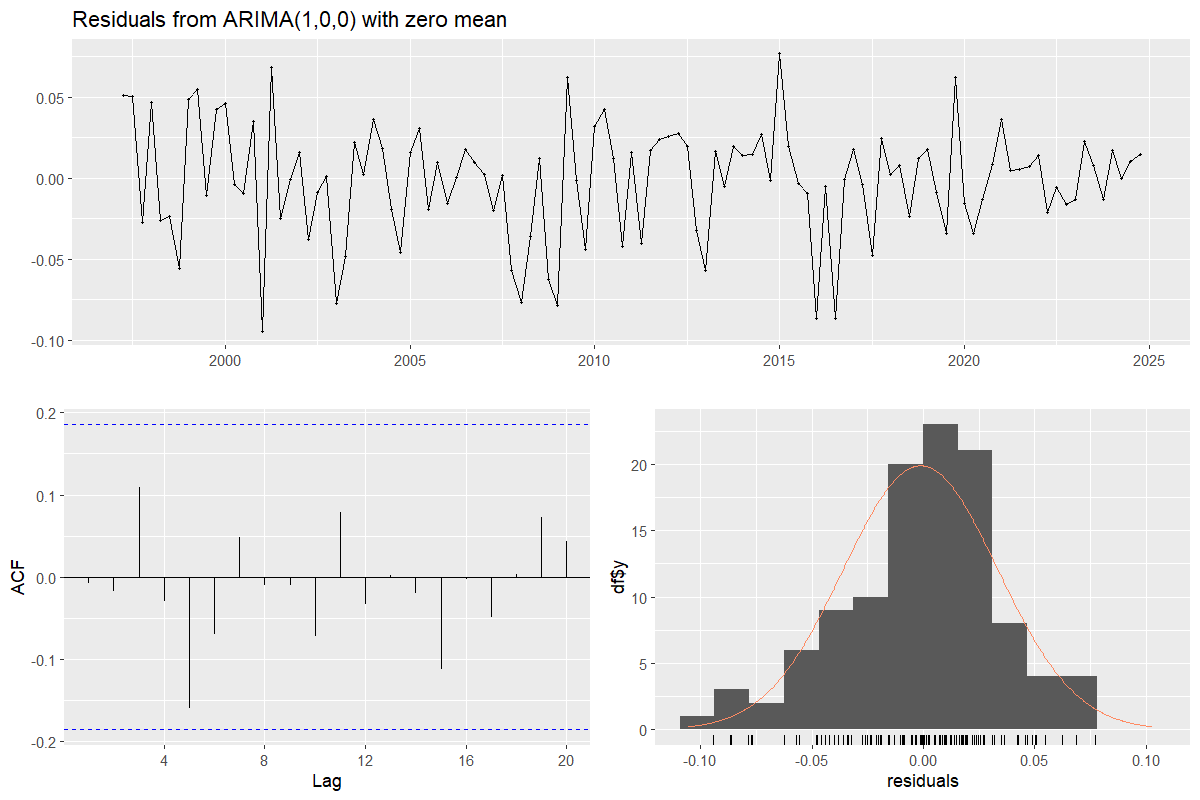
\includegraphics[width=0.8\linewidth]{../results/Exchange Rate_residuals} 

}

\caption{Model estimation - Exchange Rate}\label{fig:unnamed-chunk-12}
\end{figure}

The coefficients of the model are as follows:

\bgroup \table[H]
\centering
\caption{\label{tab:unnamed-chunk-13}Model coefficients Exchange Rate}
\centering
\begin{tabular}[t]{lrr}
\toprule
term & estimate & std.error\\
\midrule
ar1 & 0.2592112 & 0.0921888\\
\bottomrule
\end{tabular}
\endtable\egroup

\subsection*{Part 4 - Forecasting}

\textcolor{red}{We should probably focus on one series in the final report, I'll just include all so you can decide}

\textbf{GDP}

The fit of the in-sample GDP prediction is shown in the following
figure:

\begin{figure}

{\centering 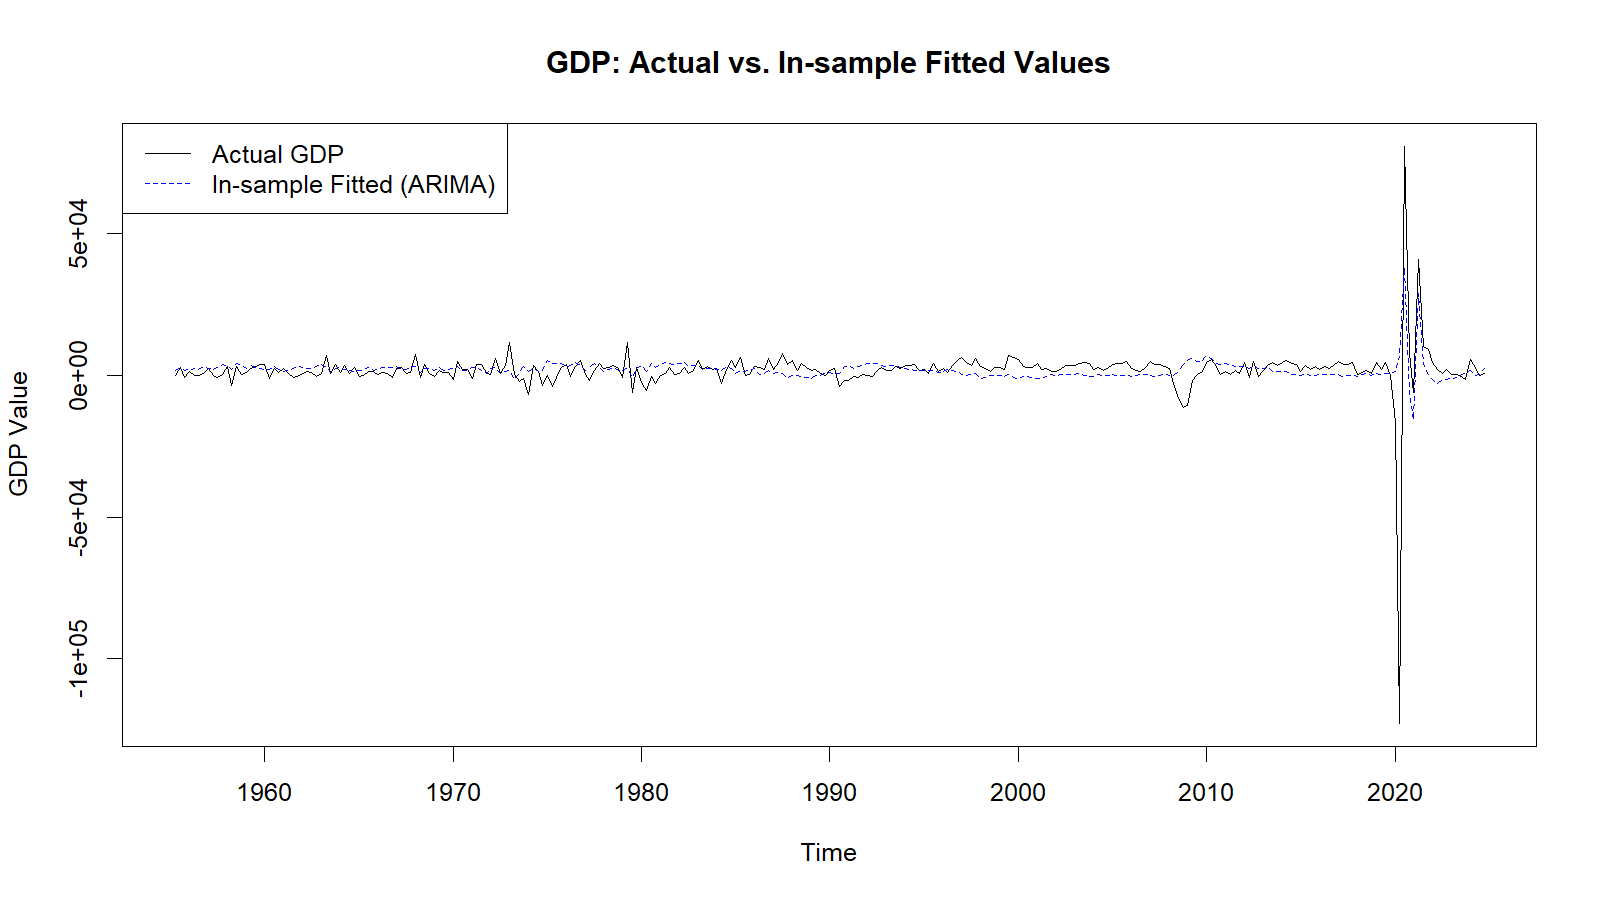
\includegraphics[width=0.8\linewidth]{../results/GDP_fitted_vs_actual} 

}

\caption{GDP - in-sample prediction}\label{fig:unnamed-chunk-14}
\end{figure}

The formal measures of the fit are estimated as:

\bgroup \table[H]
\centering
\caption{\label{tab:unnamed-chunk-15}GDP - accuracy metrics}
\centering
\begin{tabular}[t]{lrrrrrrr}
\toprule
set & ME & RMSE & MAE & MPE & MAPE & MASE & ACF1\\
\midrule
Training set & -30.63153 & 9021.217 & 3505.39 & -106.5096 & 452.5585 & 0.7699877 & -0.0027098\\
\bottomrule
\end{tabular}
\endtable\egroup

The forecast of the GDP series is:

\begin{figure}

{\centering 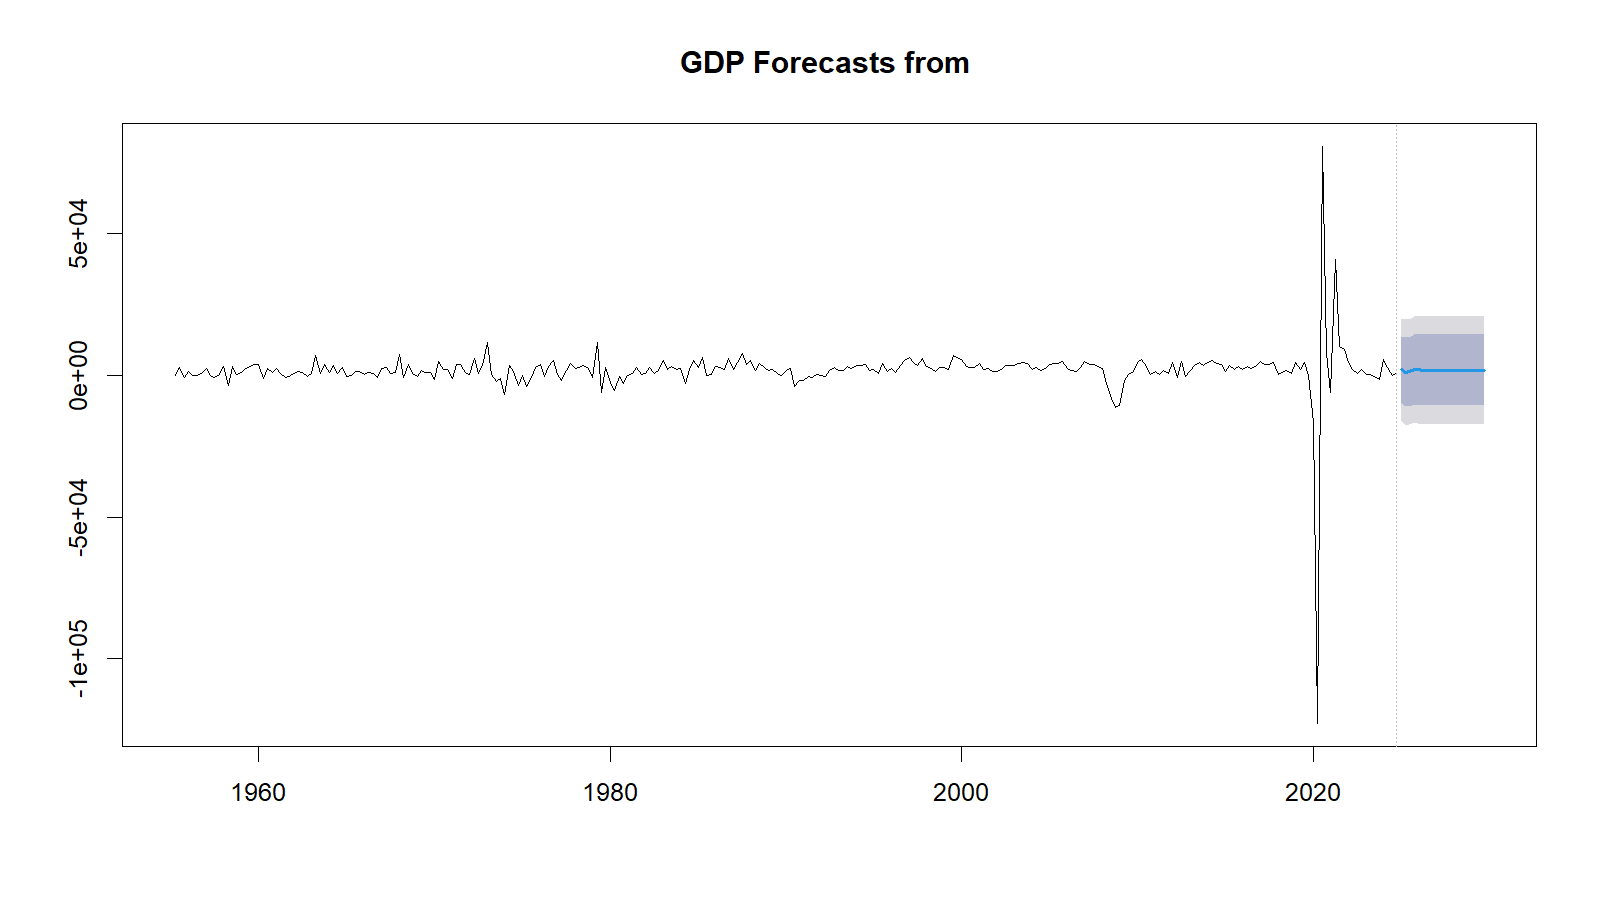
\includegraphics[width=0.8\linewidth]{../results/GDP_forecast} 

}

\caption{GDP - Forecast}\label{fig:unnamed-chunk-16}
\end{figure}

\textbf{Trade Balance}:

The in-sample fit of the Trade Balance is described by the following
metrics:

\bgroup \table[H]
\centering
\caption{\label{tab:unnamed-chunk-17}Trade Balance - accuracy metrics}
\centering
\begin{tabular}[t]{lrrrrrrr}
\toprule
set & ME & RMSE & MAE & MPE & MAPE & MASE & ACF1\\
\midrule
Training set & -196.0811 & 4513.033 & 2255.195 & Inf & Inf & 0.6855749 & 0.0055908\\
\bottomrule
\end{tabular}
\endtable\egroup

The forecast of the GDP series is:

\begin{figure}

{\centering 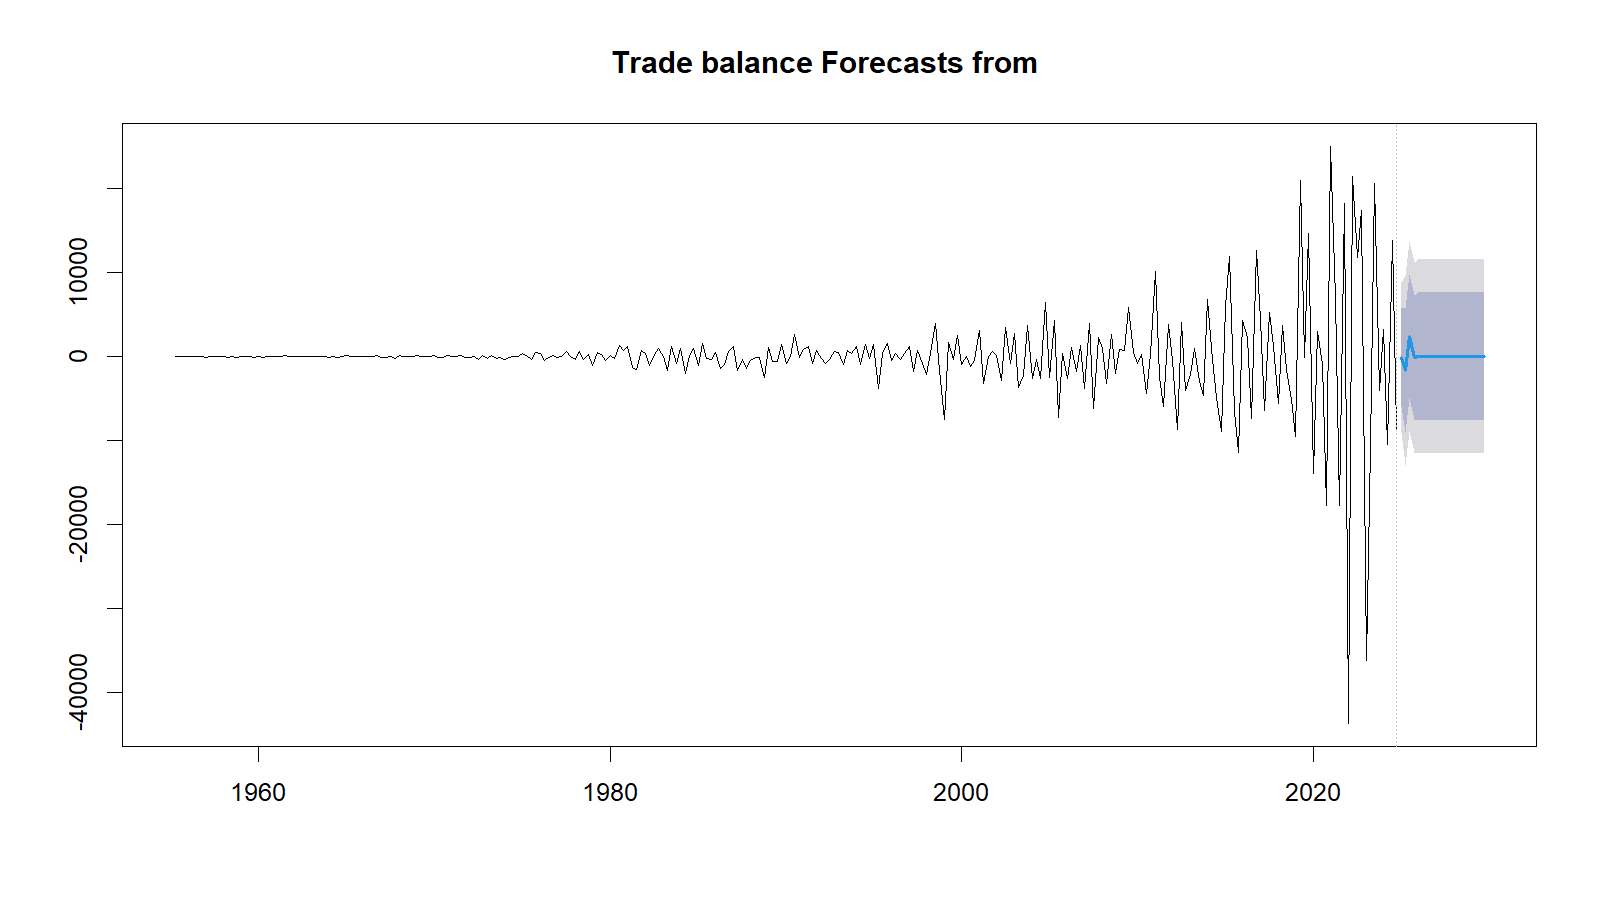
\includegraphics[width=0.8\linewidth]{../results/Trade Balance_forecast} 

}

\caption{GDP - Forecast}\label{fig:unnamed-chunk-18}
\end{figure}

\textbf{Exchange Rate}:

The in-sample fit of the Trade Balance is described by the following
metrics:

\bgroup \table[H]
\centering
\caption{\label{tab:unnamed-chunk-19}Exchange Rate - accuracy metrics}
\centering
\begin{tabular}[t]{lrrrrrrr}
\toprule
set & ME & RMSE & MAE & MPE & MAPE & MASE & ACF1\\
\midrule
Training set & -0.0011617 & 0.034616 & 0.0265389 & 137.7543 & 152.9467 & 0.6818584 & -0.0075285\\
\bottomrule
\end{tabular}
\endtable\egroup

The forecast of the GDP series is:

\begin{figure}

{\centering 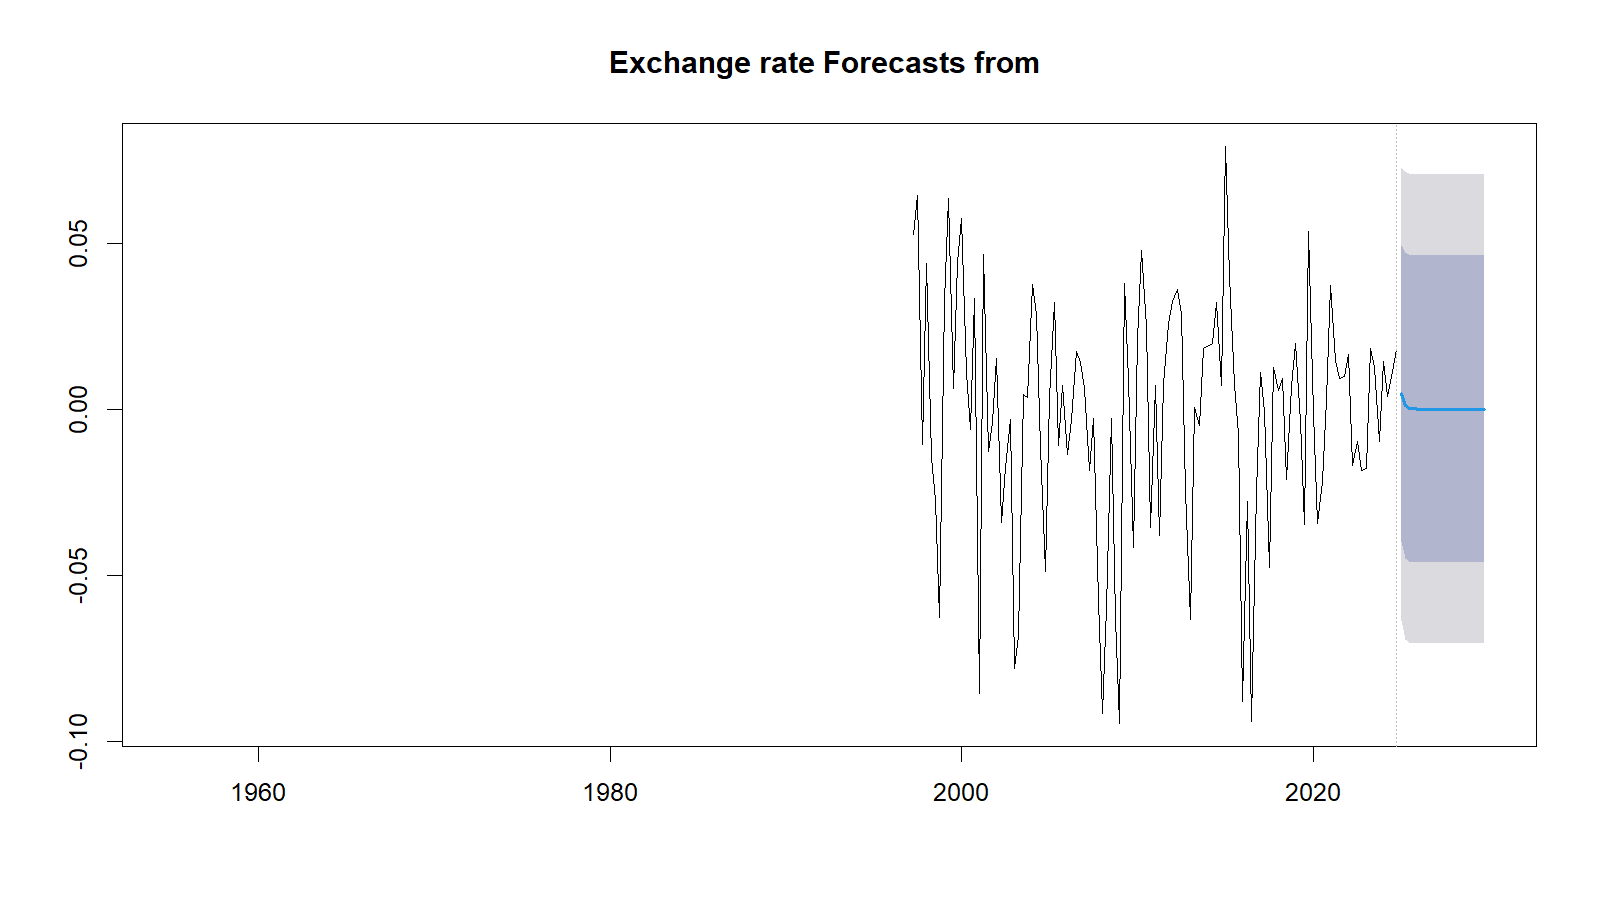
\includegraphics[width=0.8\linewidth]{../results/Exchange Rate_forecast} 

}

\caption{Exchange Rate - Forecast}\label{fig:unnamed-chunk-20}
\end{figure}

\section*{Exercise 2 - Multivariate Analysis}

\subsection*{Part 1 - Lag selection}

c.f. R script. Different tests suggest different lags as can be seen in
the following table:

\bgroup \table[H]
\centering
\caption{\label{tab:unnamed-chunk-21}Lag selection}
\centering
\begin{tabular}[t]{rrrr}
\toprule
AIC(n) & HQ(n) & SC(n) & FPE(n)\\
\midrule
7 & 1 & 1 & 7\\
\bottomrule
\end{tabular}
\endtable\egroup

We decide to use a lag of 7, ensuring better forecasting fits at the
expense of a loss of power.

\subsection*{Part 2 - Residual testing}

The test statistics for the behavior of our residuals are summarized in
the following table:

\bgroup \table[H]
\centering
\caption{\label{tab:unnamed-chunk-22}Residuals tests}
\centering
\begin{tabular}[t]{lrrr}
\toprule
Test & ChiSq & df & p.value\\
\midrule
Serial Correlation & 70.6377 & 45 & 0.0086591\\
ARCH & 290.9468 & 288 & 0.4403334\\
Normality & 7261.2574 & 6 & 0.0000000\\
\bottomrule
\end{tabular}
\endtable\egroup

\subsection*{Part 3 - VAR forecasts}

\textcolor{red}{We should probably also add an in-sample forecast as Idann and Kenan did?}

The VAR forecast of the first-differenced GDP is visualized by:

\begin{figure}

{\centering 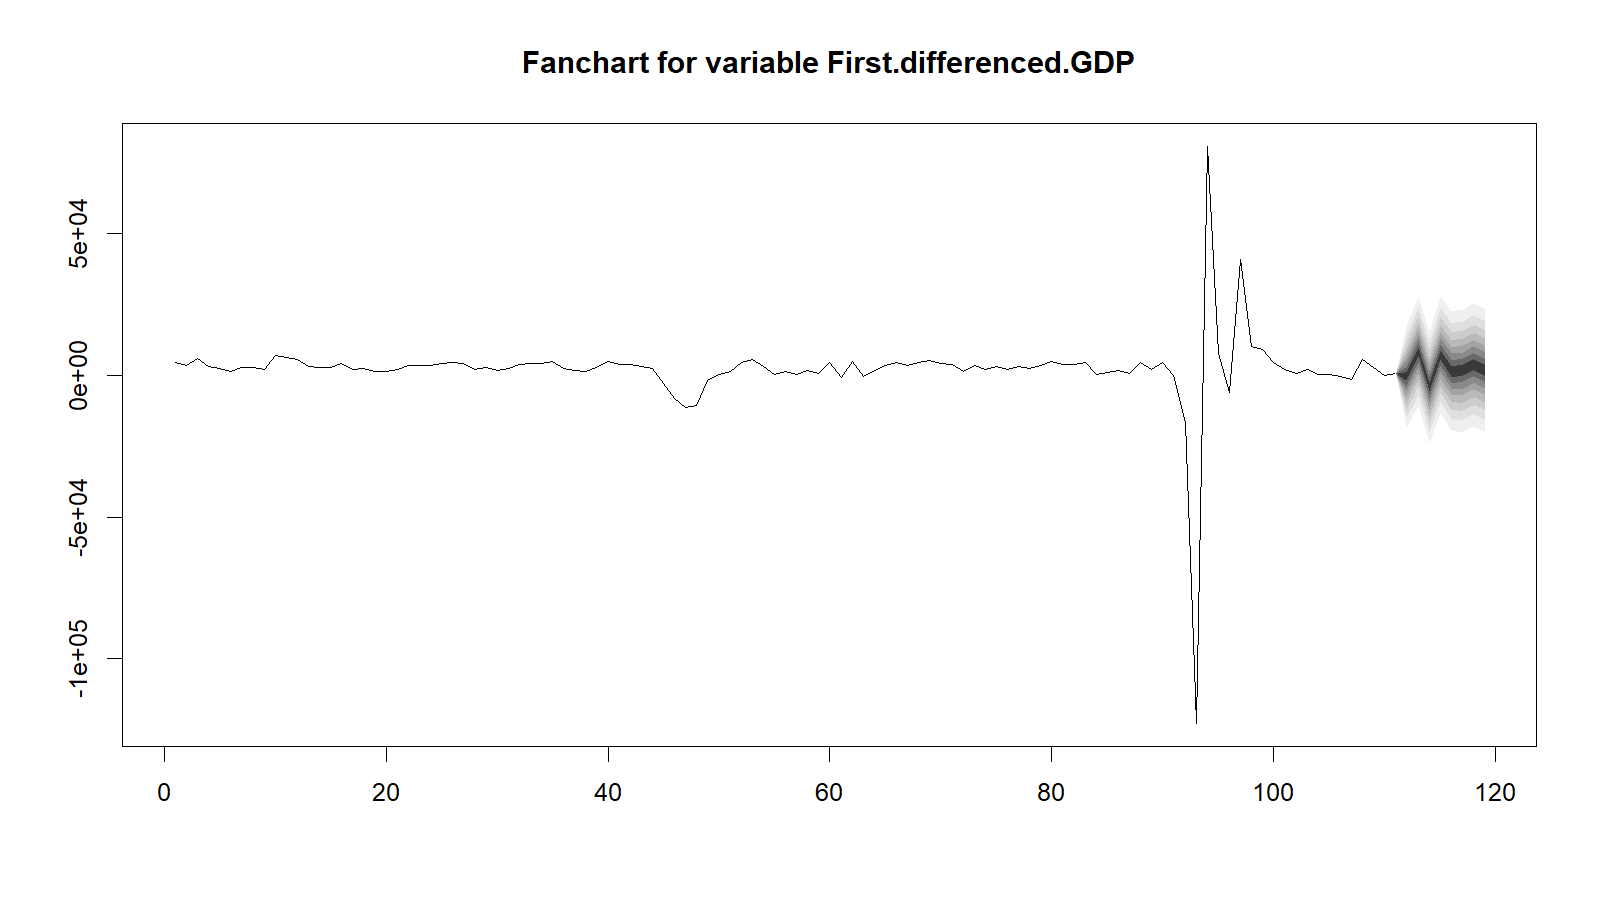
\includegraphics[width=0.8\linewidth]{../results/VAR_forecast2} 

}

\caption{GDP - VAR Forecast}\label{fig:unnamed-chunk-23}
\end{figure}

\subsection*{Part 4 - Cholesky decomposition}

\subsection*{Part 5 - Impulse response functions}

The impulse response functions for GDP are depicted as:

\begin{figure}

{\centering 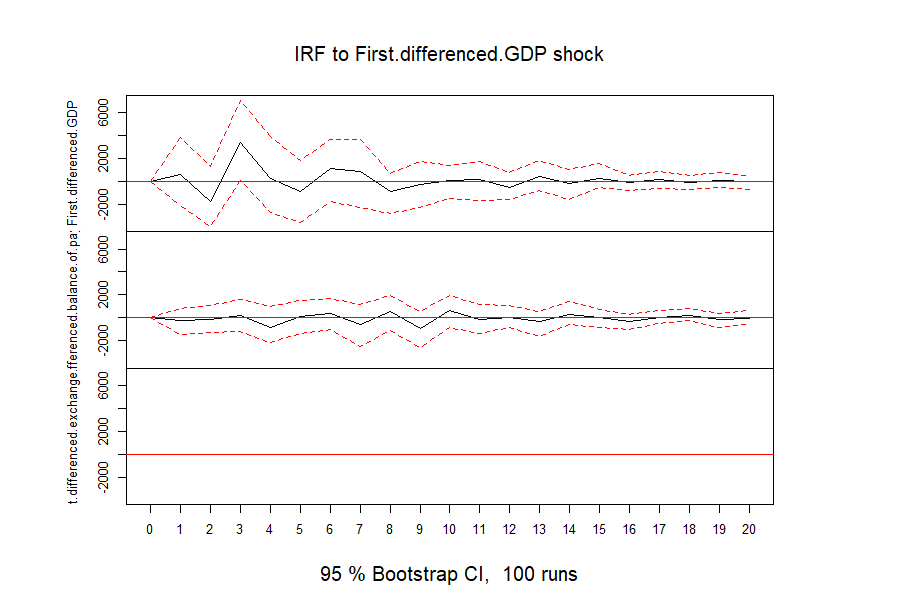
\includegraphics[width=0.8\linewidth]{../results/IRF_plots/IRF_to_First.differenced.GDP} 

}

\caption{GDP - Shock reactions}\label{fig:unnamed-chunk-24}
\end{figure}

The impulse response functions for Trade Balance are depicted as:

\begin{figure}

{\centering 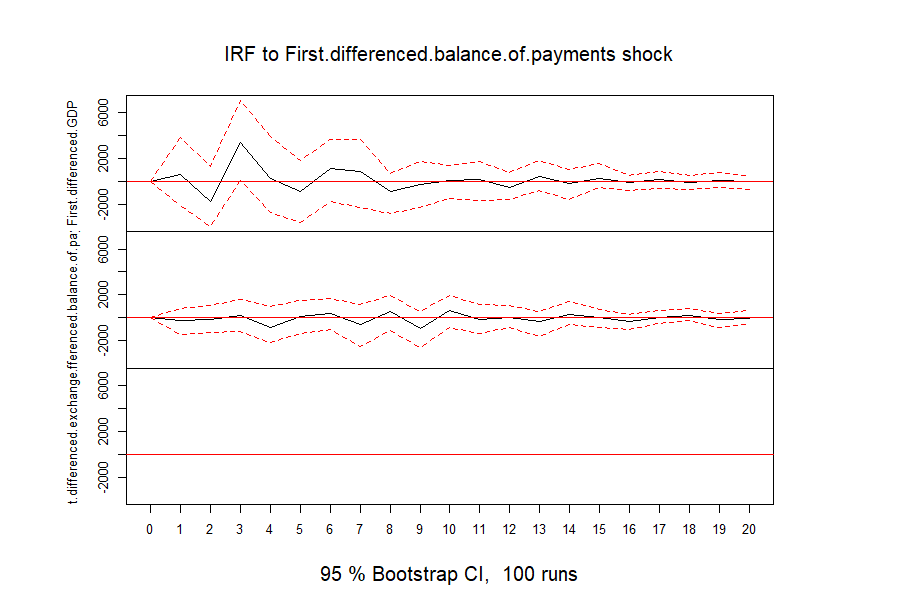
\includegraphics[width=0.8\linewidth]{../results/IRF_plots/IRF_to_First.differenced.balance.of.payments} 

}

\caption{Trade Balance - Shock reactions}\label{fig:unnamed-chunk-25}
\end{figure}

The impulse response functions for Exchange Rate are depicted as:

\begin{figure}

{\centering 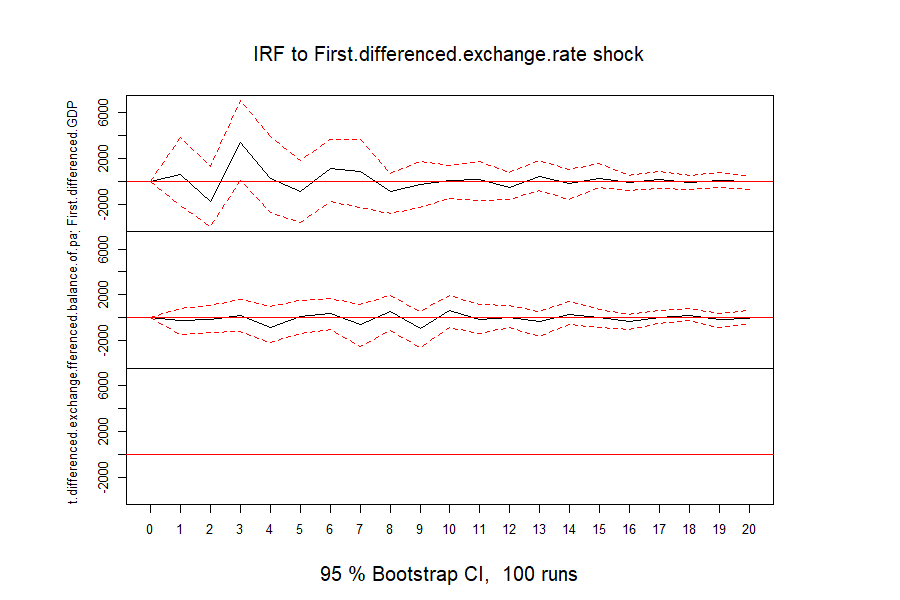
\includegraphics[width=0.8\linewidth]{../results/IRF_plots/IRF_to_First.differenced.exchange.rate} 

}

\caption{Exchange Rate - Shock reactions}\label{fig:unnamed-chunk-26}
\end{figure}

\subsection*{Part 6: Modify the ordering of the variables}

After modifying the ordering, the IRFs look as follows:

The impulse response functions for GDP are depicted as:

\begin{figure}

{\centering 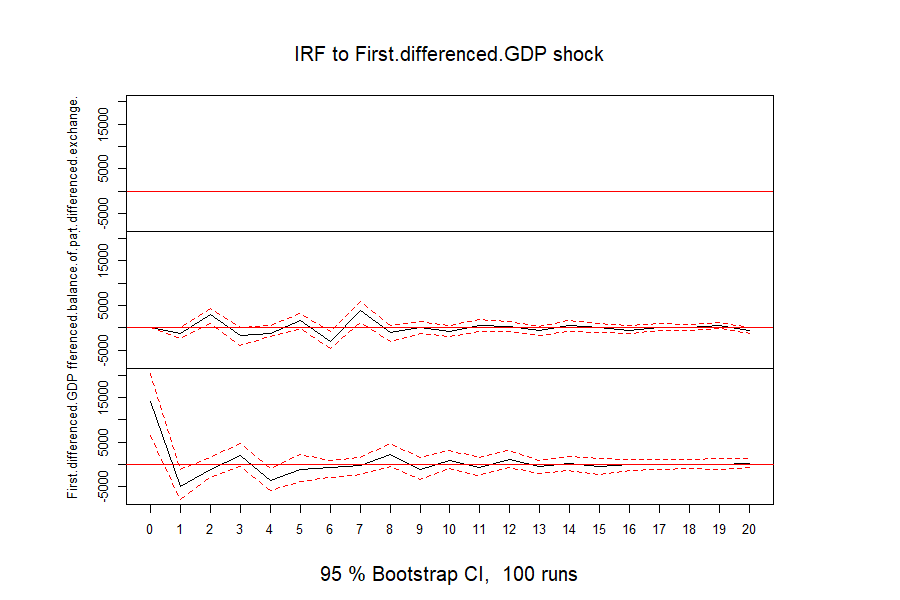
\includegraphics[width=0.8\linewidth]{../results/IRF_plots2/IRF_to_First.differenced.GDP} 

}

\caption{GDP - Shock reactions}\label{fig:unnamed-chunk-27}
\end{figure}

The impulse response functions for Trade Balance are depicted as:

\begin{figure}

{\centering 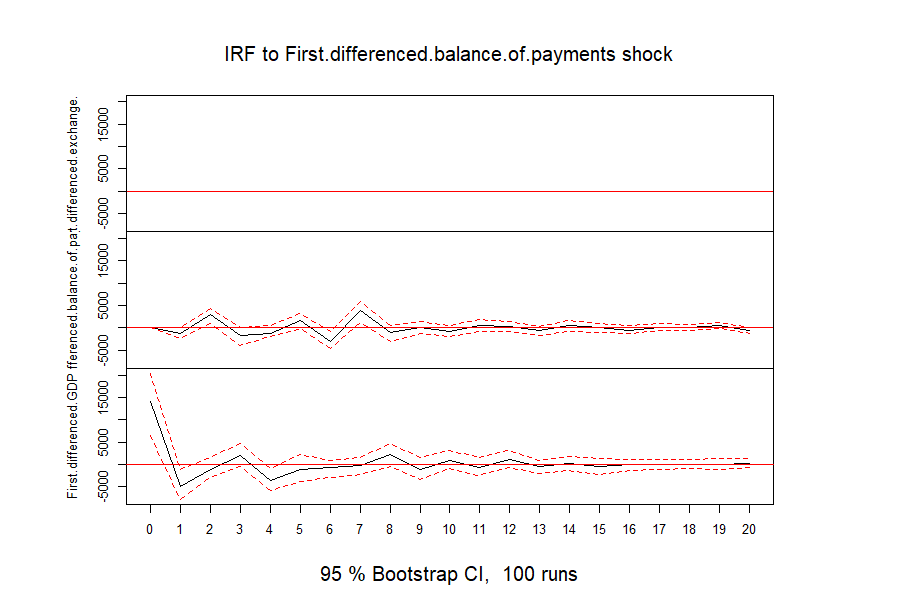
\includegraphics[width=0.8\linewidth]{../results/IRF_plots2/IRF_to_First.differenced.balance.of.payments} 

}

\caption{Trade Balance - Shock reactions}\label{fig:unnamed-chunk-28}
\end{figure}

The impulse response functions for Exchange Rate are depicted as:

\begin{figure}

{\centering 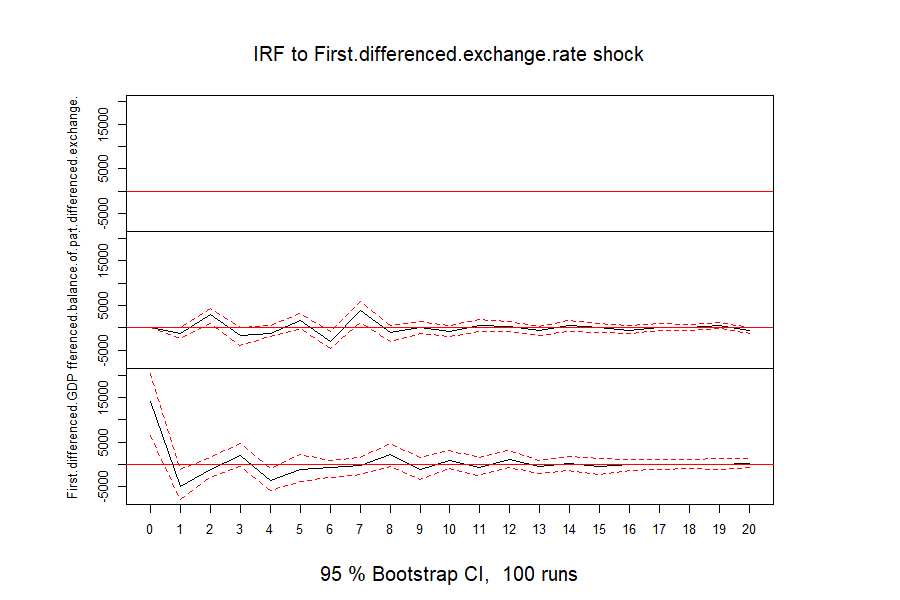
\includegraphics[width=0.8\linewidth]{../results/IRF_plots2/IRF_to_First.differenced.exchange.rate} 

}

\caption{Exchange Rate - Shock reactions}\label{fig:unnamed-chunk-29}
\end{figure}

\end{document}
